%!TEX root = ../main.tex

\chapter{Softwarearkitektur}

\RevisionsTabel{Software Arkitektur}{
		& 	 	&   \\
		& 		&   \\
		& 		&   \\
		& 	 	&   \\
}

I dette afsnit beskrives softwarearkitekturen for AVS\fxnote{AVS glossary}, som der er blevet givet indblik på i systemarkitekturen. Afsnittet skulle gerne give et indblik på det specificeret software indenfor fastlagte ramme, så udviklerne evt. kunne udarbejde det. Afsnittet indeholder dokumentation og design af de forskellige softwaredele med test på nogle af dem. \\
I afsnittet er softwaren delt ud i fire forskellige blokke som er delt op ud fra domain modelen. De fire blokke er GUI, FlexPMS, KarControl og \gls{sensoroe}. 

\section{Design og implementering af database og GUI}
I dette afsnit kommer vi ind på beskrivelsen af databasen og \glslink{gui}{gui'ens} design og implementering. Der vil være en beskrivelse af hvordan disse er anvendt i systemmet og hvordan de løser de problematikker der er stillet i kravspecifikationen.\\

\subsection{GUI}
Som udgangspunkt til at lave \glslink{gui}{gui'en} er der blevet implementeret en webside, hvor selve kommunikation mellem databasen, websiden og clienten ser ud som det kan ses i diagrammet på figur \ref{fig:web}.

\begin{figure}[H]
    \centering
    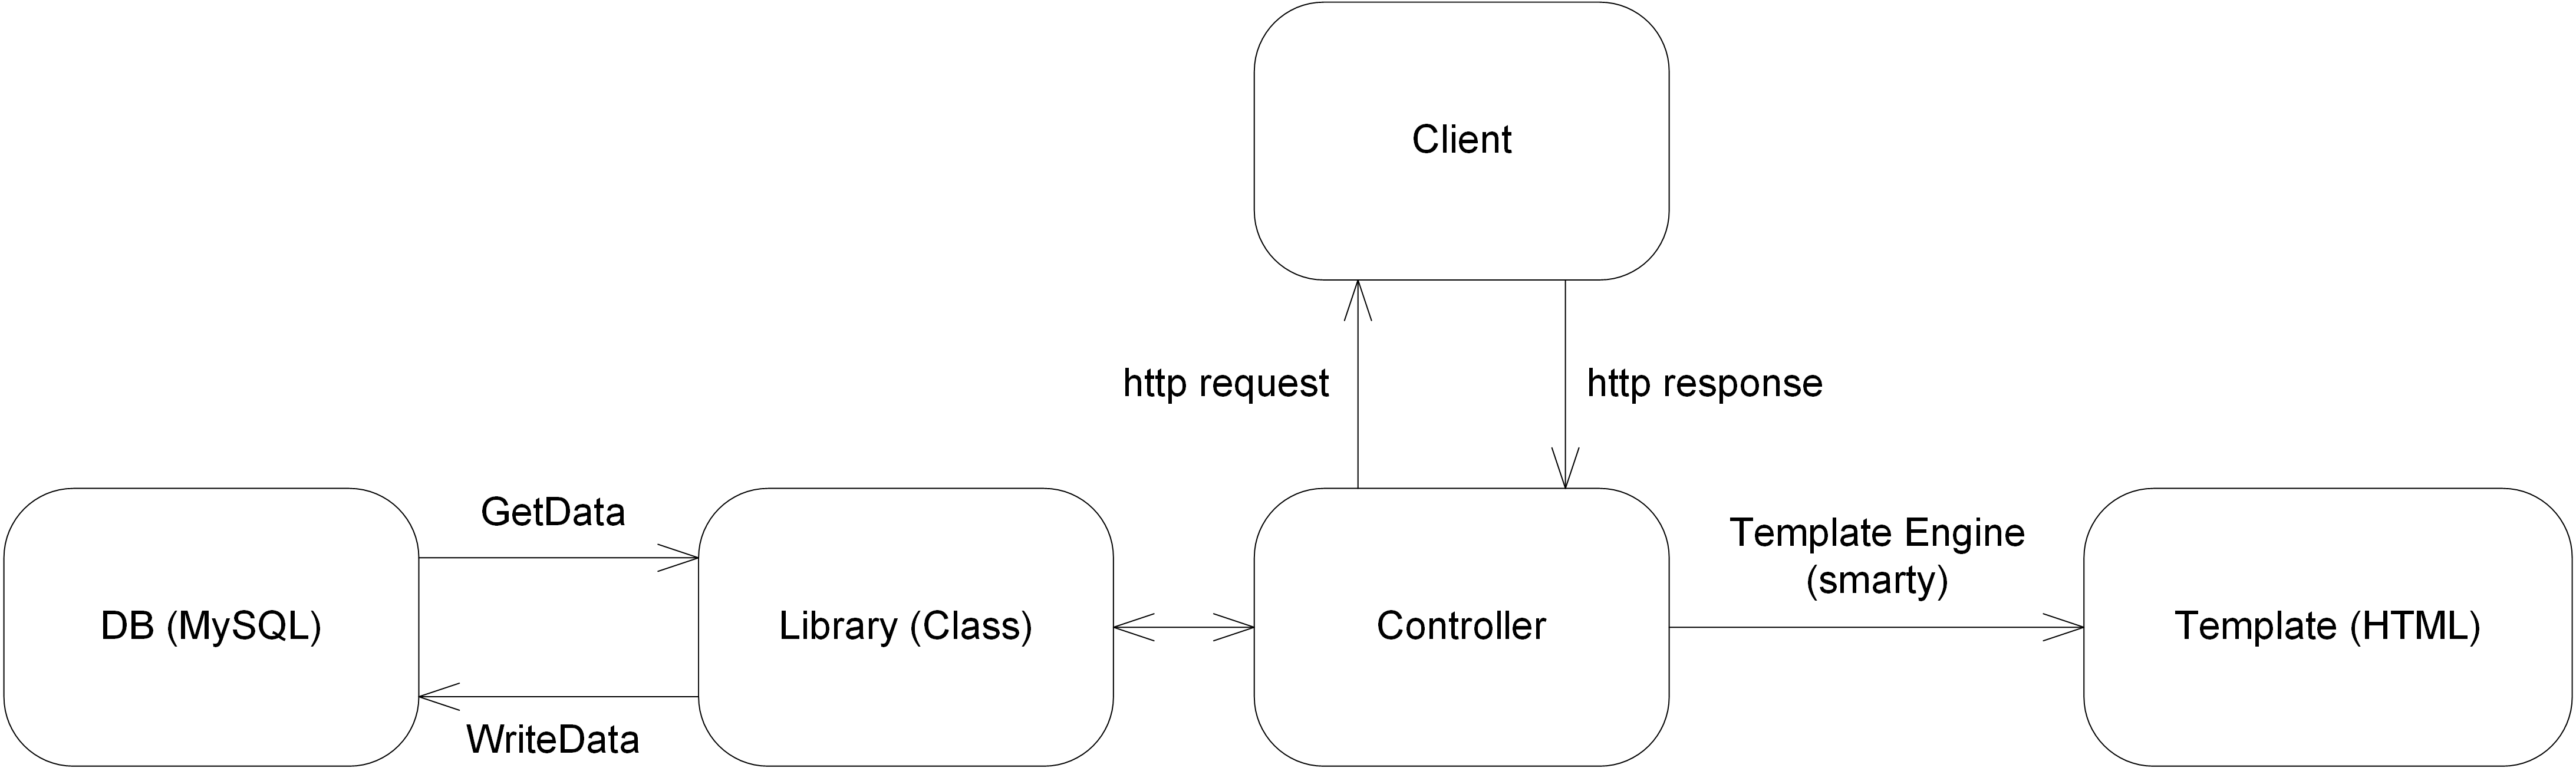
\includegraphics[width=0.8\textwidth]{SoftwareArkitektur/GUI/photo/webDiagram.png}
    \caption{Diagram over gui og databasens interaktion}
    \label{fig:web}
\end{figure}

I Libary ligger der nogle klasser så det er muligt at oprette objekter, ud fra indholdet i DB\footnote{Databasen}, inde i Controlleren. Controlleren indeholder alle PHP filerne som indeholder funktioner til at sætte websiden op og henter/opdaterer data fra databaserne.
\\\\
Under Template ligger alle HTML filerne som strukturerer indholdet på websiden og visualiserer \glslink{gui}{gui'en}. Hertil er smarty anvendt som Template Engine, det den gør, er at det tager et PHP script, udfører det, og derefter sender forskellige genererede variabler til template (HTML filerne), hvor Smarty derefter udfører forskellige opgaver med variablerne, for til slut at kompilere skabelonen til \glslink{gui}{gui'en}.
\\\\
Til template er der også anvendt Bootstrap\footnote{http://getbootstrap.com/}, som er beregnet til at gøre webudvikling lettere, da den består af HTML- og CSS- baserede design skabeloner til typografi, formularer, knapper, navigation og andre interface komponenter, samt valgfri JavaScript udvidelser.
\\\\
For at sikre at Brugeren ikke skal opdatere websiden, hver gang de vil aflæse nogle nye data eller trykke på en af knapperne er der blevet anvendt nogle jQuery AJAX metoder, som kan bruges til at udveksle data med en server og opdatere dele af en webside uden at genindlæse hele siden.

\subsection{Database}
FlexPMS databasen er blevet anvendt til at opbevare indtastede data omkring kar og sensorøerne med deres ventil og vandingsstatus, samt aflæste værdier fra de forskellige sensorer, hvor denne database kan tilgås via \glslink{gui}{gui'en}. MySQL er databaseformatet der er valgt, og valget bunder i at denne har alle de kvaliteter systembeskrivelsen og kravspecifikationen foreskriver. Desuden er softwaren til etablering af en sådan server gratis, veldokumenteret og nem at gå til.
\\\\
Databasen indeholder nogle forskellig tabeller som er bestemt ud fra de krav vi skulle tilfredsstilles i kravspecifikation og det design der er lavet i systemarkitekturen. Disse tabeller, deres kolonnenavne og deres datatype er illustreret i figur \ref{fig:DB}. 

\begin{figure}[H]
    \centering
    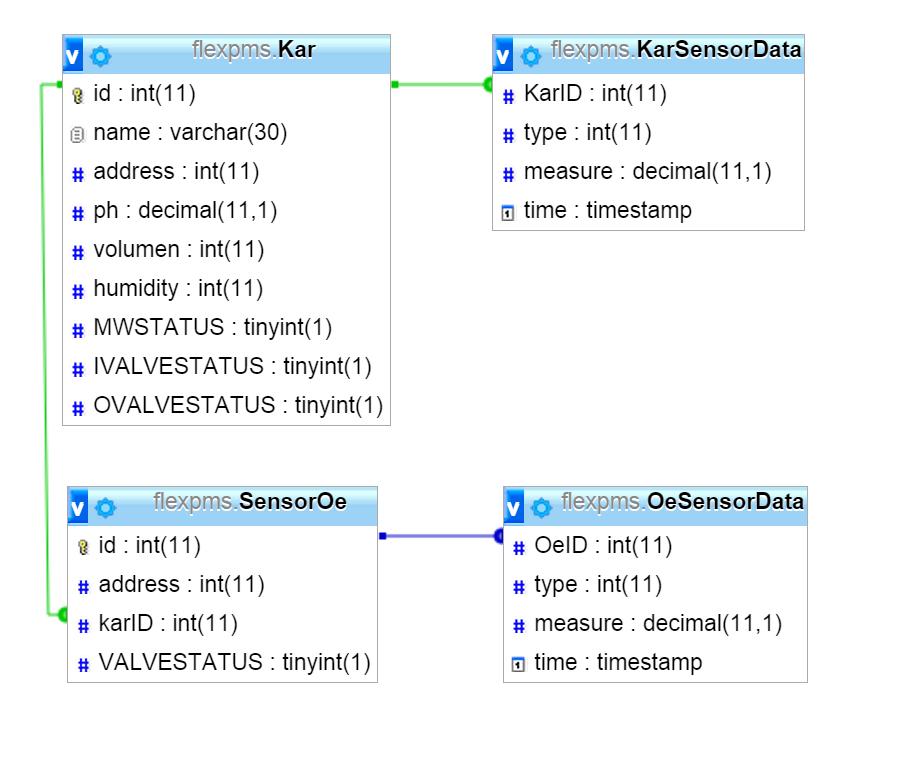
\includegraphics[width=0.7\textwidth]{SoftwareArkitektur/GUI/photo/DB_diagram.PNG}
    \caption{Diagram over FlexPMS databasen}
    \label{fig:DB}
\end{figure}

Som det fremgår af diagrammet kender tabellerne til hinanden, det gør de via deres id. Hver \gls{sensoroe} og \gls{kar} har et unikt id for at sikre man kan differentiere mellem dem. Grunden til at dette er vigtigt er fordi at det sikre at data ikke bliver dubleret, ført forkert ind i tabellerne, eller har nogle forkerte interaktioner.
\\\\
En kort beskrivelse af tabellerne og deres kolonner i databasen følger:

\subsubsection{Kar}
Kar indeholder alle kar, deres kar data, som brugeren har oprettet og status for dens ventiler. Alle kar har et navn og adresse med de data som Brugeren ønsker at karet skal have. Kolonnenavnene er beskrevet i tabel \ref{table:kar_kol}.

\begin{table}[H]
\center
\footnotesize
	\begin{tabular}{ | >{\raggedright}p{2.5cm} | >{\raggedright\arraybackslash}p{9.5cm} | }
    \hline
    \vskip 1px \textbf{Kolonnenavn} 	\vskip 0.5px 			& \vskip 0.5px \textbf{Beskrivelse} \vskip 1px 	\\ \hline
    \textit{id} 						& Et unikt id for hver kar tabellen indeholder   						\\ \hline
   	\textit{name} 						& Navnet på karet   													\\ \hline
   	\textit{adresse}	 				& Adressen til karet    												\\ \hline
   	\textit{ph} 						& Den indtastede pH-værdi som Brugeren ønsker    						\\ \hline
   	\textit{volumen} 					& Det vandniveau/antal liter vand som Brugeren ønsker i karet 			\\ \hline
   	\textit{humidity} 					& Den jordfugtighed brugeren ønsker ved \glslink{sensoroe}{Sensor Øerne}\\ \hline
   	\vskip 4pt \textit{MWSTATUS} 		& \vskip 1px
											\begin{minipage}{9cm}
   												Status for manuel vanding:	
    											\begin{itemize}
   													\item 1: Manuel vanding er startet
   													\item 0: Manuel vanding er stoppet
   												\end{itemize}
   												\vskip 1px
 											\end{minipage}   													\\ \hline
 	\vskip 4pt \textit{IVALVESTATUS} 		& \vskip 1px 
											\begin{minipage}{9cm}
   												Status for indløbsventil:	
    											\begin{itemize}
   													\item 1: Indløbsventilen er åben
   													\item 0: Indløbsventilen er lukket
   												\end{itemize}
   												\vskip 1px
 											\end{minipage}   													\\ \hline
 	\vskip 4pt \textit{OVALVESTATUS} 		& \vskip 1px 
											\begin{minipage}{9cm}
   												Status for afløbsventil:	
    											\begin{itemize}
   													\item 1: Afløbsventilen er åben
   													\item 0: Afløbsventilen er lukket
   												\end{itemize}
   												\vskip 1px
 											\end{minipage}   
 																												\\ \hline
\end{tabular}
\caption{Beskrivelser af kolonnenavne for tabellen Kar}
\label{table:kar_kol}
\end{table}


\subsubsection{SensorOe} 
SensorOe indeholder alle Sensor Øer, deres data brugeren har oprette og status for dens ventil. hver Sensor Ø har også et KarID så man kan se hvilket Kar de hører til. Kolonnenavnene er beskrevet i tabel \ref{table:SensorOe_kol}.
\begin{table}[H]
\center
\footnotesize
	\begin{tabular}{ | >{\raggedright}p{2.5cm} | >{\raggedright\arraybackslash}p{9.5cm} | }
    \hline
    \vskip 1px \textbf{Kolonnenavn} \vskip 0.5px & \vskip 0.5px \textbf{Beskrivelse}  \vskip 1px 				\\ \hline
    \textit{id} 						& Et unikt id for hver Sensor Ø tabellen indeholder   					\\ \hline
   	\textit{adresse} 					& Adressen til Sensor Ø    													\\ \hline
   	\textit{KarID}	 					& En reference til det Kars id som Sensor Øen sidder på   				\\ \hline
   	\vskip 4pt \textit{VALVESTATUS} 	& \vskip 1px
											\begin{minipage}{9cm}
   												Status ventilen ved Sensor Øen:	
    											\begin{itemize}
   													\item 1: Ventilen er åben
   													\item 0: Ventilen er lukket
   												\end{itemize}
   												\vskip 1px
 											\end{minipage}   													\\ \hline
\end{tabular}
\caption{Beskrivelser af kolonnenavne for tabellen SensorOe}
\label{table:SensorOe_kol}
\end{table}


\subsubsection{KarSensorData}
KarSensorData indholder alle de målte værdier ved hver kar, derfor har de et KarID, som man kan se hvilken værdi det tilhører. Her indikerer type hvilken slags måling det er, hvor measure værdien der bliver målt. Ydermere er der time der angiver tiden hvor de tilhørende data blev sat ind, på den måde kan man altid tilgå de nyeste data. Kolonnenavnene er beskrevet i tabel \ref{table:karSensorData_kol}.
\begin{table}[H]
\center
\footnotesize
	\begin{tabular}{ | >{\raggedright}p{2.5cm} | >{\raggedright\arraybackslash}p{9.5cm} | }
    \hline
    \vskip 1px \textbf{Kolonnenavn} \vskip 0.5px & \vskip 0.5px \textbf{Beskrivelse}  \vskip 1px 				\\ \hline
    \textit{KarID} 						& En reference til det Kars id der bliver målt på    					\\ \hline
    \vskip 4pt \textit{type} 			& \vskip 1px
											\begin{minipage}{9cm}
   												Hvilken type sensor der er lavet måling på:	
    											\begin{itemize}
   													\item 1: pH-værdi på væsken i karret
   													\item 2: Vandniveau/Antal liter der bliver tilført til karet
   													\item 9: Gennemsnittet af jordfugtigheden målt ved Sensor Øerne 
   												\end{itemize}
   												\vskip 1px
 											\end{minipage}   													\\ \hline
   	\textit{measure} 					& Den aflæste sensor værdi 												\\ \hline
   	\textit{time}	 					& Tidspunktet værdien blev sat in i tabelen				 				\\ \hline
\end{tabular}
\caption{Beskrivelser af kolonnenavne for tabellen KarSensorData}
\label{table:karSensorData_kol}
\end{table}


\subsubsection{OeSensorData}
OeSensorData minder meget om KarSensorData men indholder alle de målte værdier ved hver \gls{sensoroe} og derfor har de et OeID. Kolonnenavnene er beskrevet i tabel \ref{table:oeSensorData_kol}.

\begin{table}[H]
\center
\footnotesize
	\begin{tabular}{ | >{\raggedright}p{2.5cm} | >{\raggedright\arraybackslash}p{9.5cm} | }
    \hline
    \vskip 1px \textbf{Kolonnenavn} \vskip 0.5px & \vskip 0.5px \textbf{Beskrivelse}  \vskip 1px 				\\ \hline
    \textit{OeID} 						& En reference til det Sensor Øs id der bliver målt på    				\\ \hline
    \vskip 4pt \textit{type} 			& \vskip 1px
											\begin{minipage}{9cm}
   												Hvilken type sensor der er lavet måling på:	
    											\begin{itemize}
   													\item 9: Jordfugtigheden målt ved Sensor Øen 
   												\end{itemize}
   												\vskip 1px
 											\end{minipage}   													\\ \hline
   	\textit{measure} 					& Den aflæste sensor værdi 												\\ \hline
   	\textit{time}	 					& Tidspunktet værdien blev sat in i tabelen				 				\\ \hline
\end{tabular}
\caption{Beskrivelser af kolonnenavne for tabellen KarSensorData}
\label{table:oeSensorData_kol}
\end{table}


\section{FlexPMS}
Programmet FlexPMS er designet til at være bindeled mellem brugergrænsefladen og kar/sensorø styringerne, der til får programmet nogle opgaver der hedder sig at programmet skal op sample data og gemme dette i databasen, samt holde en log af det opsamlede data. Programmet skal også facilitere kommunikationen fra brugergrænsefladen til kar/sensorø når der for eksempel bliver bedt om at starte en vanding i brugergrænsefladen eller det ønskes at styre ventiler. FlexPMS kunne også udvides således at programmet selv kan bestemme hvornår der skal vandes baseret på de målinger der er fortaget.\\\\

Her under har vi et pakke diagram der viser hvordan de forskellige dele af systemet arbejder sammen, hver enkelt pakke er beskrevet i følgende afsnit hvor der også kan findes klasse beskrivelser af de klasser der bor i de individuelle pakker.

\PakkeDiagram{1}{FlexPMS}{FlexPMS}

\subsection{Threading}
FlexPMS er dybt afhængig af trådteknologi. De tre store komponenter, Socket serveren, Bridge og Kar bus, kører parallelt i hver sin tråd. Trådene kommunikerer med hinanden gennem et event-baseret beskedsystem. Al trådhåndtering er skrevet specifikt til at køre på Linux, og FlexPMS er derfor ikke understøttet af andre operativsystemer.

\KlasseDiagram{0.5}{FlexPMS}{Thread}

\subsubsection{Thread}
\textit{Thread} er en abstrakt basis-klasse for alle klasser, som skal afvikles i sin egen tråd. Ved at nedarve fra \textit{Thread} kan en klasse nøjes med at implementere en \textKode{run()} metode, der kaldes, når tråden startes via \textKode{start()}. Tråden lever indtil \textKode{run()} returnerer, eller indtil der kaldes \textKode{cancel()} på en tråd, og tråden dør. \textit{Thread} er udelukkende skrevet til at understøtte pthread på Linux.

\StateDiagram{0.6}{FlexPMS}{Thread}

\subsubsection{Arkitekturspecifikke metoder}

\funk{void start()}{Starter tråden}{Ingenting}
{}

\funk{void cancel()}{Stopper tråden, hvis annullering er slået til, ellers gør funktionen ingenting. Tråden stoppes først når der stødes på et såkaldt cancellation point. Kun tråden selv kan tillade eller forbyde annullering}{Ingenting}
{}

\funk{void join()}{Blokerende kald, som ikke returnerer før tråden er færdig med eksekvering}{Ingenting}
{}

\funk{virtual void run()}{Abstrakt metode, som kaldes når tråden startes. Tråden lever så længe run() er under afvikling, eller indtil den annulleres}{Ingenting}
{}

\funk{static void* run\_thread(void* arg)}{C-style funktion hvori tråden startes. Denne funktion kaldes af \textKode{start()} og kalder til gengæld \textKode{run()} på Thread-objektet}{Ingenting}
{
\funkArg{arg}{En pointer til det Thread-objekt, som skal køres i en tråd}
}

\funk{void enable\_cancel()}{Tillader annullering af tråden, så tråden kan stoppes hvis \textKode{cancel()} kaldes}{Ingenting}
{}

\funk{void disable\_cancel()}{Forbyder annullering af tråden, så hvis \textKode{cancel()} kaldes ignoreres det}{Ingenting}
{}

\funk{void ssleep(unsigned int sec)}{Lægger tråden til at sove i et antal sekunder (minimum)}{Ingenting}
{
\funkArg{sec}{Antal sekunder tråden minimum skal sove i}
}

\funk{void msleep(unsigned int msec)}{Lægger tråden til at sove i et antal millisekunder (minimum))}{Ingenting}
{
\funkArg{msec}{Antal millisekunder tråden minimum skal sove i}
}


\subsection{Event-baseret beskedsystem}
FlexPMS er opbygget af adskillige tråde, som alle kan snakke sammen ved at sende beskeder til hinanden. Trådene håndterer udelukkende beskeder sendt til dem udefra, og står derfor udelukkende i blokerende kald til en besked-kø, så længe de ikke er ved at håndtere en indkommende besked. Trådene nedarver fra \textit{MessageThread} og har pointers til de tråde, som de skal kunne sende beskeder til.

\KlasseDiagram{1}{FlexPMS}{EventSystem}


\subsubsection{MessageThread}
Klassen, som er en specialisering af \textit{Thread}, stiller funktionalitet til rådighed til at indgå i det event-baserede beskedsystem. Ved at nedarve fra \textit{MessageThread} bliver en klasse til en modtager af beskeder, og kan i den forbindelse nøjes med at implementere en \textKode{dispatch()} metode, som kaldes hver gang tråden modtager en besked via dens send() metode. \textKode{dispatch()} modtager to argumenter; et event-ID samt en pointer til et \textit{Message}-objekt, der evt. kan være \textKode{NULL}. Dispatch bør overholde reglen om, at kalde en funktion til at håndtere beskeden alt efter hvilket event-ID den modtager.\\\\

\textKode{send()} tager ligeledes to argumenter; et event-ID samt en pointer til et \textit{Message}-objekt. Det er afsenderen, som skal allokere \textit{Message}-objektet, men \textit{MessageThread} sørger selv for, at de-allokere det efter \textKode{dispatch()} er kaldt hos modtageren.\\\\

\SekvensDiagram{1}{FlexPMS}{MessageThread}

\textit{MessageThread} laver udelukkende blokerende kald til dens besked-kø, og dermed undgår vi, at stå og bruge CPU-tid i løkker, som ikke udfører noget. Det betyder, at alle klasse som nedarver fra \textit{MessageThread} udelukkende håndterer events sendt til dem udefra. På den måde lægges tråde til at sove så længe der ikke er noget at lave, og programmet vil bruge minimalt CPU-tid.


\StateDiagram{0.5}{FlexPMS}{MessageThread}

\subsubsection{Arkitekturspecifikke metoder}

\funk{virtual void init()}{Abstrakt metode, som kaldes inden der begyndes at hente beskeder fra beskedkøen}{Ingenting}
{}

\funk{void send(unsigned long id, Message* msg = NULL)}{Lægger en besked i trådens beskedkø}{Ingenting}
{
\funkArg{id}{Et ID, som beskriver det event der sendes}
\funkArg{msg}{En pointer til et \textit{Message}-objekt, som kan holde på yderligere data}
}

\funk{virtual void dispatch(unsigned long event\_id, Message* msg))}{Abstrakt metode, som kaldes hver gang tråden modtager en besked. Metoden skal overskrives af klasser, som nedarver fra \textit{MessageThread} til at håndtere indkommende beskeder}{Ingenting}
{
\funkArg{event\_id}{Et ID, som beskriver det event der sendes}
\funkArg{msg}{En pointer til et \textit{Message}-objekt, som kan holde på yderligere data. Kan være \textKode{NULL}}
}


\subsubsection{MessageQueue}

Klassen er en FIFO kø, som er trådsikret, dvs. sikret mod de problemer der kan opstå i forbindelse med at tilgå den parallelt fra forskellige tråde. \textit{MessageQueue} er implementeret via en queue (fra STL) og benytter sig at pthread’s \textit{mutex} og \textit{conditional variable} til at synkronisere mellem tråde. \textit{MessageQueue} er udelukkende brugt internt i \textit{MessageThread}.

\begin{figure}[H]
	\centering
	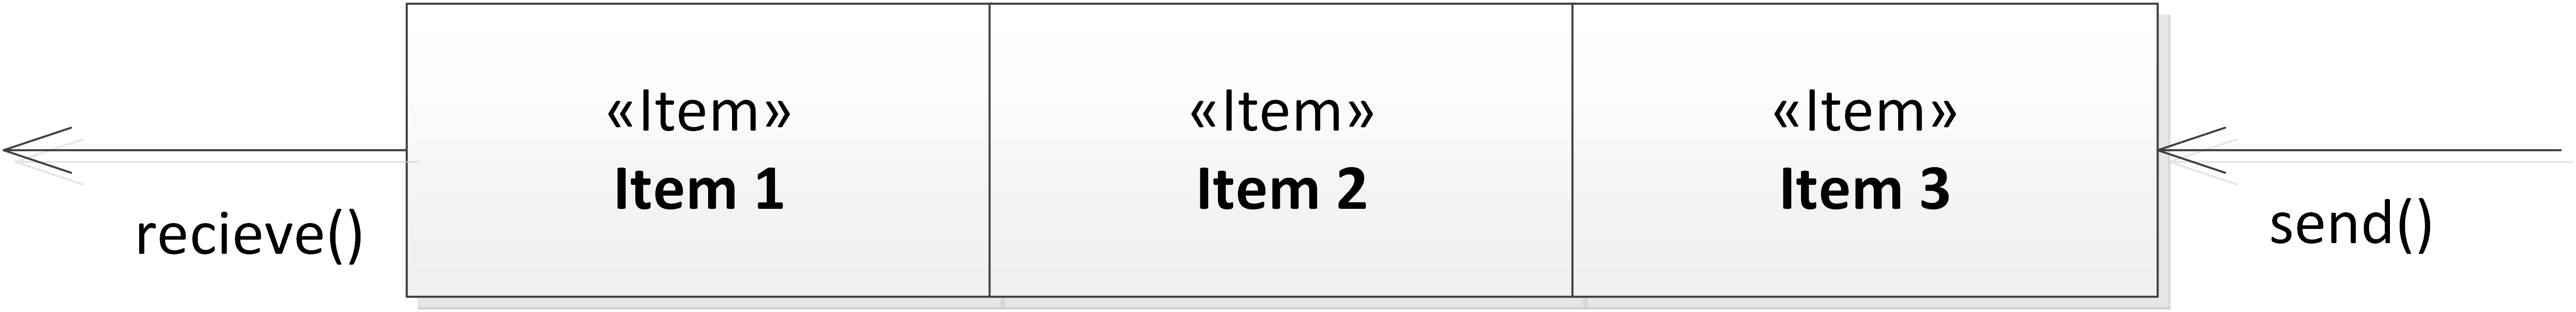
\includegraphics[scale=1]{SoftwareArkitektur/FlexPMS/Diagrammer/MessageQueue_FIFO.png}
	\caption{MessageQueue FIFO}
	\label{photo:MessageQueueFIFO}
\end{figure}


\subsubsection{Arkitekturspecifikke metoder}

\funk{void send(unsigned long id, Message* msg = NULL)}{Putter en besked i køen}{Ingenting}
{
\funkArg{id}{Event-ID som skal puttes i køen}
\funkArg{msg}{Pointer til \textit{Message}-objekt, som skal puttes i køen}
}

\funk{Message* recieve(unsigned long\& id)}{Henter den næste besked fra køen. Hvis køen er tom, så blokerer funktionen indtil der bliver puttet noget i køen via \textKode{send()}}{Ingenting}
{
\funkArg{id}{Funktionen skriver event-ID til denne variabel}
}

\subsubsection{Item}

\textit{Struct}, som udelukkende benyttes internt i \textit{MessageQueue}. Den holder på event ID'er og \textit{Message}-objekter, og er den type, der placeres i køen.


\subsubsection{Message}

\textit{Message} gør det muligt at medsende informationer (ud over et event-ID), når tråde kommunikerer med hinanden. Klassen \textit{Message} indeholder en sender attribut, som er en pointer til den \textit{MessageThread}, der sendte beskeden. sender gør det derfor muligt for \textit{MessageThread}'s at svare på beskeder direkte tilbage til afsenderen.\\\\

Alt efter hvilke data man vil sende med en besked kan man nedarve fra \textit{Message} og tilføje flere attributter.  Der er lavet specialiseringer af \textit{Message} hvor det har været nødvendigt at sende information mellem tråde.\\\\

\textbf{KarBusMessage}\\
Klassen er en specialisering af \textit{Message} og indeholder – ud over \textKode{sender} – en kar attribut, som er en pointer til det \textit{Kar}-objekt, der skal sendes data til. Grunden til, at kar kun er implementeret på \textit{KarBusMessage} er, at det altid er relevant at have information med omkring hvilket kar der skal sendes instrukser til når der kommunikeres mellem \textit{Bridge} og \textit{KarBus}, hvorimod dette ikke er nødvendigt når der kommunikeres mellem \textit{Bridge} og \textit{SocketClient}.\\\\

Der er adskillige specialiseringer af \textit{KarBusMessage}, som benyttes alt afhængigt af beskeden (event-ID).\\\\

\textbf{SessionMessage}\\
Klassen er en specialisering af \textit{Message} og bruges i forbindelse med, at \textit{SocketClient} skal registrere sig selv hos \textit{Bridge}. \textit{Bridge} sender en \textit{SessionMessage} til \textit{SocketClient} når klienten er registreret. Klassen indeholder en \textKode{session\_id} attribut.\\\\

\textbf{GuiMessage}\\
Klassen er en specialisering af \textit{Message} og indeholder – ud over sender – flere attributter, som bruges i forbindelse med kommunikation mellem \textit{SocketClient} og \textit{Bridge}. Klienten (webserveren) har mulighed for at sende kommandoer, som er specifikke for enten Kar eller SensorØ, og det er derfor relevant at tilføje disse attributter på \textit{GuiMessage}. Klassen indeholder desuden også en \textKode{session\_id} attribut, så Bridge ved hvilken klient den skal sende til i tilfælde, hvor svar til klienten er nødvendigt.


\subsection{Logging}
Vi benytter logging til at gemme alle handlinger, som har med sensorer og aktuatorer at gøre. Loggen skrives til en fil med tidsstempel. Det er udelukkende Bridge, som skriver til loggen.\\\\

Følgende handlinger bliver logget:

\begin{itemize}
\item Der modtages data fra sensorer på et Kar
\item Der modtages data fra sensorer på en SensorØ
\item Der modtages information om, hvorvidt en ventil på et Kar er blevet åbnet eller lukket
\item Der modtages information om, hvorvidt en ventil på en SensorØ er blevet åbnet eller lukket
\item Der modtages information om en pumpes status (slukket eller tændt/pumpe-hastighed)
\item Når GUI anmoder om at starte manuel vanding logges der, for hver SensorØ, at dens ventil blev anmodet om at åbne. Der logges, at Karrets pumpe blev anmodet om at startet
\item Når GUI anmoder om at stoppe manuel vanding logges der, for hver SensorØ, at dens ventil blev anmodet om at lukke. Der logges, at Karrets pumpe blev anmodet om at stoppet
\item Når GUI anmoder om at åbne eller lukke indløbs- eller afløbsventil på et Kar
\end{itemize}

Alt andet debugging skrives til FlexPMS' stdout. Det er derfor muligt at omdirigere stdout til en fil for at logge samtlige debugging udskrifter.


\KlasseDiagram{0.5}{FlexPMS}{Logging}

\subsubsection{Log}
Klassen benyttes til at skrive til loggen. Den er implementeret vha. Singleton, dvs. at kun én instans af klassen kan eksistere på tværs af hele FlexPMS. Instansen bliver oprettet gennem kald fra main.cpp, hvorefter den lever som en statisk member på klassen Log så længe FlexPMS kører.\\\\

Hver gang der skrives til loggen tilføjes tidsstempel samt linjeskift efter teksten.

\subsubsection{Arkitekturspecifikke metoder}

\funk{static Log* getInstance()}{Funktionen returnerer en instans af Log. Hvis en instans endnu ikke er blevet oprettet, så oprettes den først}{Instans af klassen Log}
{}

\funk{void write(std::string line)}{Funktionen skriver en linje til logfilen}{Ingenting}
{
\funkArg{line}{Tekst, som skal skrives til logfilen}
}



\subsection{Database og domænemodeller}
Systemet benytter sig af en MySQL database. For at forbinde til databasen gennem FlexPMS benyttes det officielle bibliotek fra MySQL til at forbinde gennem C++, \textit{mysqlcppconn}. FlexPMS kører i øvrigt ikke transaktionsbaseret.\\\\

Tilgang til databasen er pakket ind i forskellige domæneklasser, som håndterer de lavpraktiske SQL forespørgsler. Domæneklasserne stiller en højniveau-grænseflade til rådighed for resten af programmet.\\\\

Forbindelsen til databasen oprettes i main.cpp når FlexPMS starter, og holdes åben så længe programmet lever. Der gives en pointer til DB-forbindelsen med til \textit{Bridge}, som er den eneste klasse, der arbejder med domæneklasserne.


\KlasseDiagram{1}{FlexPMS}{Database}

\subsubsection{Kar}
Klassen repræsenterer ét Kar, og stiller en højniveau-grænseflade til rådighed, til at opdatere værdier for et kar i databasen.

\subsubsection{Arkitekturspecifikke metoder}

\funk{void set\_mwstatus(bool s)}{Funktionen sætter status for manuel vanding}{Ingenting}
{
\funkArg{s}{Status for manuel vanding. \textKode{True} er tændt, \textKode{False} er slukket}
}

\funk{void set\_ivalvestatus(bool s)}{Funktionen sætter status for, hvorvidt indløbsventilen er åben eller lukket}{Ingenting}
{
\funkArg{s}{Status for indløbsventilen. \textKode{True} er åben, \textKode{False} er lukket}
}

\funk{void set\_ovalvestatus(bool s)}{Funktionen sætter status for, hvorvidt afløbsventilen er åben eller lukket}{Ingenting}
{
\funkArg{s}{Status for afløbsventilen. \textKode{True} er åben, \textKode{False} er lukket}
}

\funk{void add\_sensor\_data(int type, double value)}{Funktionen registrerer data fra en sensor koblet til karret}{Ingenting}
{
\funkArg{type}{Sensor type ID}
\funkArg{value}{Den målte værdi}
}


\subsubsection{SensorOe}
Klassen repræsenterer én sensor ø, stiller en højniveau-grænseflade til rådighed, til at opdatere værdier for en sensor ø i databasen.

\subsubsection{Arkitekturspecifikke metoder}

\funk{void set\_valvestatus(bool s)}{Funktionen sætter status for, hvorvidt ventilen er åben eller lukket}{Ingenting}
{
\funkArg{s}{Status for ventilen. \textKode{True} er åben, \textKode{False} er lukket}
}

\funk{void add\_sensor\_data(int type, double value)}{Funktionen registrerer data fra en sensor koblet til sensor ø’en}{Ingenting}
{
\funkArg{type}{Sensor type ID}
\funkArg{value}{Den målte værdi}
}



\subsubsection{DBContainer}
\textit{DBContainer} er en abstrakt basis-klasse for alle klasser, som skal holde på lister af objekter. \textit{DBContainer} implementerer funktionalitet til at tilgå en række af resultater fra et databaseudtræk. Den nedarvede klasse skal selv implementere databaseudtrækket via \textKode{reload()} metoden, men får derudover stillet alle andre nødvendige metoder til rådighed til at tilgå resultaterne.\\\\

\textit{DBContainer} er implementeret med et C++ map (fra STL), hvor nøglen er et unikt ID og værdien er et objekt, som repræsenterer én række i databasen. Da \textit{DBContainer} er en template-klasse kan objekterne være af hvilken som helst type. Nøglerne skal dog være af typen \textKode{unsigned int}.\\\\

Nedarvede klasser skal implementere \textKode{reload()} metoden, som kaldes umiddelbart efter at objektet er blevet instantieret. \textKode{reload()} metodens formål er, at hente data fra databasen, instantiere objekter og tilføje dem til mappet.

\subsubsection{Arkitekturspecifikke metoder}

\funk{T* get(unsigned int id)}{Returnerer en pointer til objektet med nøglen id. Hvis nøglen ikke findes returneres \textKode{NULL}}{En pointer til objektet med nøglen \textKode{id}. Hvis nøglen ikke findes returneres \textKode{NULL}}
{
\funkArg{id}{Primærnøglen på det objekt, som skal søges efter}
}

\funk{bool contains(unsigned int id)}{Tjekker hvorvidt et objekt eksisterer i mappet}{\textKode{True} hvis objektet eksisterer, ellers \textKode{False}}
{
\funkArg{id}{Primærnøglen på det objekt, som skal søges efter}
}

\funk{const unsigned int size()}{Tæller antallet af objekter i mappet}{Antallet af objekter i mappet}
{}

\funk{void iter()}{Forbereder objektet til at blive itereret over fra begyndelsen}{Ingenting}
{}

\funk{T* next()}{Returnerer det næste objekt i en iteration. Kald \textKode{iter()} inden iterationen begyndes for at være sikker på, at der startes fra begyndelsen}{Det næste objekt af typen \textKode{T}}
{}

\funk{virtual void reload() = 0}{Abstrakt metode, som skal implementeres af nedarvede klasser. Dens formål er, at hente data fra databasen og putte det ind i mappet. Funktionen kaldes umiddelbart efter at \textit{DBContainer} bliver instantieret}{Ingenting}
{}


\subsubsection{KarContainer}
Klasse, som er en specialisering af \textit{DBContainer}, giver mulighed for at arbejde med en liste af \textit{Kar}-objekter.


\subsubsection{SensoeOeContainer}
Klasse, som er en specialisering af \textit{DBContainer}, giver mulighed for at arbejde med en liste af \textit{SensorOe}-objekter.

\subsection{Socket server}
Denne del af FlexPMS giver GUI'en adgang til at kommunikere direkte med FlexPMS via TCP/IP, og bruges til at informere FlexPMS om handlinger, som skal startes eller stoppes, og er den eneste direkte vej for GUI at kommunikere med FlexPMS.



\KlasseDiagram{1}{FlexPMS}{SocketServer}

\subsubsection{SocketServer}
Klassen, som er en specialisering af \textit{Thread}, har det ene formål, at lytte efter indkommende forbindelser fra GUI’en over TCP/IP. Når \textit{SocketServer} modtager en ny forbindelse startes en ny tråd, \textit{SocketClient}, hvori al kommunikation mellem GUI og FlexPMS foregår. Når \textit{SocketServer} har oprettet og startet en ny \textit{SocketClient} mister den al forbindelse til den, og kender derfor ikke til åbne forbindelser til klienter.\\\\

Serveren lytter på adresse 127.0.0.1 (localhost) port 5555.

\StateDiagram{0.5}{FlexPMS}{SocketServer}


\subsubsection{SocketClient}

\textit{SocketClient}, som er en specialisering af \textit{MessageThread}, håndterer al kommunikation mellem klienten (GUI) og Bridge. Den bliver oprettet af \textit{SocketServer} når der kommer en ny indkommende forbindelse. Den består desuden af en privat \textit{SocketReader} klasse, hvis eneste formål er, at læse data fra en socket. \textit{SocketReader} er implementeret, så der kan laves blokerende læse-kald fra socket, og på den måde undgår vi, at \textit{SocketClient} står i løkker hvor den laver to ikke-blokerende kald (henholdsvis at læse fra socket, samt at læse fra sin egen besked-kø).\\\\

\textit{SocketClient} modtager beskeder fra enten \textit{SocketReader} eller Bridge. \textit{SocketReader} sender beskeder når der enten er modtaget nyt data fra klienten, eller når klienten lukker forbindelsen. Bridge sender beskeder når der enten er data at sende til klienten, eller når forbindelsen til klienten skal lukkes.\\\\

Når \textit{SocketClient} oprettes får den givet en file-descriptor til den socket, som den skal læse fra og skrive til. Lige efter at klassen er blevet oprettet, registrerer den sig hos Bridge, der svarer tilbage med et unikt sessions ID, som skal gives med hver gang \textit{SocketClient} sender beskeder til Bridge. Bridge bruger dette ID til at identificere klienter i tilfælde, hvor der skal sendes et svar tilbage til klienten. Bridge har derfor en intern mapning af, hvilke sessions sessions ID'er der hører til hvilke \textit{SocketClient} klasser. Det er med andre ord Bridge, og ikke \textit{SocketServer}, som holder styr over åbne forbindelser til klienter.\\\\

Når \textit{SocketClient} er blevet registreret hos Bridge starter den \textit{SocketReader}, som begynder at læse data fra socket. Herefter kan en udveksling af data mellem GUI og FlexPMS begynde.\\\\

\textit{SocketClient} dør når én af tre handlinger finder sted:

\begin{enumerate}
\item \textit{SocketReader} fik en fejl, da den forsøgte at læse fra socket
\item \textit{SocketClient} fik en fejl, da den forsøgte at skrive til socket
\item Bridge giver besked om, at forbindelsen til klienten skal lukkes 
\end{enumerate}

I de to første tilfælde skal \textit{SocketClient} give Bridge besked om, at forbindelse til klienten er død, og \textit{SocketClient} skal stoppes. I det sidste tilfælde skal \textit{SocketClient} reagere på beskeden og stoppe sig selv. Herefter ved Bridge, at den skal fjerne alle spor af \textit{SocketClient} klassen (herunder session og brugt hukommelse).

\StateDiagram{1}{FlexPMS}{SocketClient}

Nedenfor ses et sekvensdiagram, som illustrerer \textit{SocketClient}'s livscyklus.

\SekvensDiagram{1}{FlexPMS}{SocketClient}

\subsection{Bridge}
\textit{Controller}, der består af \textit{Bridge}, som er en specialisering af \textit{MessageThread}, er den centrale controller i FlexPMS. Den kommunikerer med både GUI og KarBus, og håndterer al den logik der ligger ind imellem. Det er også Bridge, der håndterer timing-baserede events som f.eks. at poll'e data fra kar. Det er også Bridge, der tilgår databasen gennem domænemodeller.

\KlasseDiagram{0.85}{FlexPMS}{Controller}

\subsubsection{Bridge}


\textbf{Sessions}\\
Når Bridge modtager en forespørgsel fra en \textit{SocketClient} om at blive registreret, så tildeler Bridge den forespørgende \textit{SocketClient} det næste ledige sessions ID. Herefter kan \textit{SocketClient} begynde at sende beskeder til \textit{Bridge}, som videreformidler beskederne til \textit{KarBus}. Beskeden til \textit{KarBus} skulle indeholde et sessions ID på den forespørgende \textit{SocketClient}, så i tilfælde af, at \textit{SocketClient} skulle have svar, kunne \textit{KarBus} sende ID'et med tilbage til \textit{Bridge}, som kunne identificere hvilken \textit{SocketClient} den skulle sende svaret til. Vi fik dog aldrig brug for at sende svar tilbage til \textit{SocketClient}, så sessions ID'er er ikke blevet implementeret i kommunikationen mellem \textit{Bridge} og \textit{KarBus}.\\\\

Se Figur \ref{fig:SocketClient_SekvensDiagram} for en \textit{SocketClient}'s livscyklus, som inkluderer registrering med sessioner.\\\\

\textbf{Events}\\

\textit{Bridge} kan modtage følgende events fra \textit{SocketClient}:

\begin{itemize}
\item \textKode{E\_HELLO} håndteres af \textKode{handle\_hello()}
\item \textKode{E\_BYE} håndteres af \textKode{handle\_bye()}
\item \textKode{E\_START\_WATERING} håndteres af \textKode{handle\_start\_watering()}
\item \textKode{E\_STOP\_WATERING} håndteres af \textKode{handle\_stop\_watering()}
\item \textKode{E\_OVALVE\_OPEN} håndteres af \textKode{handle\_ovalve\_open()}
\item \textKode{E\_OVALVE\_CLOSE} håndteres af \textKode{handle\_ovalve\_close()}
\item \textKode{E\_IVALVE\_OPEN} håndteres af \textKode{handle\_ivalve\_open()}
\item \textKode{E\_IVALVE\_CLOSE} håndteres af \textKode{handle\_ivalve\_close()}
\end{itemize}

\textit{Bridge} kan modtage følgende events fra \textit{KarBus}:

\begin{itemize}
\item \textKode{E\_KAR\_READY\_STATE} håndteres af \textKode{handle\_kar\_ready\_state()}
\item \textKode{E\_KAR\_OE\_LIST} håndteres af \textKode{handle\_kar\_oe\_list()}
\item \textKode{E\_KAR\_SENSOR\_DATA} håndteres af \textKode{handle\_kar\_sensor\_data()}
\item \textKode{E\_KAR\_VALVE\_STATE} håndteres af \textKode{handle\_kar\_valve\_state()}
\item \textKode{E\_KAR\_PUMP\_STATE} håndteres af \textKode{handle\_kar\_pump\_state()}
\item \textKode{E\_OE\_VALVE\_STATE} håndteres af \textKode{handle\_oe\_valve\_state()}
\item \textKode{E\_OE\_SENSOR\_DATA} håndteres af \textKode{handle\_oe\_sensor\_data()}
\end{itemize}

\textbf{KarPinger}\\
\textit{KarPinger}, som er en specialisering af \textit{Thread}, har det ene formål at sende et PING-event til \textit{Bridge} hvert 10. sekund. PING-eventet starter processen med at polle sensor-data fra både Kar og Sensor Ø'er.

\SekvensDiagram{1}{FlexPMS}{KarPinger}


\subsection{Kar Kommunikation}
Kar kommunikations pakken er ansvarlig for at sende beskeder til kar styringen den står altså for grænsefalden ud til sensor og aktautore igennem kommunikation til kar styringen. Den består af 3 klasser der er illustreret  i diagrammet herunder:

\KlasseDiagram{1}{FlexPMS}{KarBus}

\subsubsection{KarBus klassen}
Den klasse interfacer med resten af flexpms igennem den event baserede kommunikation der driver systemet klassen har således sin egen message kø og tilsvarende event handlers. KarBus har også en RS485 instans og en Protokol instans i sig, Protokol klassen er implementeringen af Karbus protokollen som KarBus klassen bruger til at sende beskeder til karret, RS485 klassen er ikke direkte brugt af KarBus.


\subsubsection{Funktionsbeskrivelser}
Her er de funktioner der er nævnt for karbus i figur \ref{fig:KarBus_KlasseDiagram} beskrevet
\funk{void eHandleKarReady(MKarReady* msg)}{Denne eventhandler kalder den relavante funktion i protokol klassen og stykker det relavante svar sammen hvis der bliver returneret et svar fra RS485 bussen}{ingenting}
{
\funkArg{msg}{En besked om at tjekke at karret er klar til kommunikation}
}

\funk{void eHandleKarGetSensorData(MKarGetSensorData* msg)}{Denne eventhandler kalder den relavante funktion i protokol klassen og stykker det relavante svar sammen hvis der bliver returneret et svar fra RS485 bussen}{ingenting}
{
\funkArg{msg}{En besked om at hente sensor data fra karret}
}

\funk{void eHandleKarSetPumpState(MKarSetPumpState* msg)}{Denne eventhandler kalder den relavante funktion i protokol klassen og stykker det relavante svar sammen hvis der bliver returneret et svar fra RS485 bussen}{ingenting}
{
\funkArg{msg}{En besked om at styre pumpen så denne køre med den hastighed der er indehold i beskeden}
}

\funk{void eHandleKarSetPumpState(MKarSetPumpState* msg)}{Denne eventhandler kalder den relavante funktion i protokol klassen og stykker det relavante svar sammen hvis der bliver returneret et svar fra RS485 bussen}{ingenting}
{
\funkArg{msg}{En besked om at styre pumpen så denne køre med den hastighed der er indehold i beskeden}
}

\funk{void eHandleOeGetSensorData(MOeGetSensorData* msg)}{Denne eventhandler kalder den relavante funktion i protokol klassen og stykker det relavante svar sammen hvis der bliver returneret et svar fra RS485 bussen}{ingenting}
{
\funkArg{msg}{En besked om hente data fra sensor'øen}
}

\funk{void eHandleOeSetValve(MOeSetValveSate* msg)}{Denne eventhandler kalder den relavante funktion i protokol klassen og stykker det relavante svar sammen hvis der bliver returneret et svar fra RS485 bussen}{ingenting}
{
\funkArg{msg}{En besked at styre ventilen på sensor'øen}
}

\funk{void eHandleOeGetSensorType(MOeGetSensorType* msg)}{Denne eventhandler kalder den relavante funktion i protokol klassen og stykker det relavante svar sammen hvis der bliver returneret et svar fra RS485 bussen}{ingenting}
{
\funkArg{msg}{En besked at få afvide hvilken sensortype der er koblet til en bestemt adresse}
}

\funk{void eHandleKarSetValve(MKarSetValveState* msg)}{Denne eventhandler kalder den relavante funktion i protokol klassen og stykker det relavante svar sammen hvis der bliver returneret et svar fra RS485 bussen}{ingenting}
{
\funkArg{msg}{En besked at styre ventilen på karret den kan indeholde om det er afløb eller indløb der skal styres}
}

\funk{void eHandleKarGetOeList(MKarGetOeLIst* msg)}{Denne eventhandler kalder den relavante funktion i protokol klassen og stykker det relavante svar sammen hvis der bliver returneret et svar fra RS485 bussen}{ingenting}
{
\funkArg{msg}{En besked om at få en list af ø'er der er tilkoblet et kar}
}

\funk{void eHandleKarOpretOe(MKarSetOpretOe* msg)}{Denne eventhandler kalder den relavante funktion i protokol klassen og stykker det relavante svar sammen hvis der bliver returneret et svar fra RS485 bussen}{ingenting}
{
\funkArg{msg}{En besked om at oprette en ø der bliver knyttet til et kar}
}

\subsubsection{Protokol klassen}
Denne klasse er en direkte implementering af karbus protokollen det vil sige at den har en funktion per besked der er i protokollen det gør at det er nemt at tilføje beskeder til protokollen men også at andre dele af koden er mindre afhængige af protokollen og hvordan denne håndtere kommunikationen til hardware.
Klassen har en pointer til RS485 klassen som den bruger til at sende beskederne med, RS485 kunne for så vidt erstattes af en anden klasse hvis det var ønskeligt at kommunikere på anden vis end via RS485. 

\subsubsection{Funktionsbeskrivelser}
Her er de funktioner der er nævnt for protokol klassen i figur \ref{fig:KarBus_KlasseDiagram} beskrevet
\funk{bool sendAndReceive()}{Denne funktion kalder send og modtage funktionerne i RS485 klassen}{Der bliver returneret true hvis en besked blev modtaget ellers false}
{
}

\funk{bool getKarRdy(unsigned char karID, unsigned char\& karState)}{Denne funktion gør en besked klar til at forspørge om et kar er klar til kommunikation derefter venter den indtil der er modtaget en besked med \textKode{sendAndReceive} funktionen returtypen sætte alt efter om der modtages en besked}{Der bliver returneret true hvis en besked blev modtaget ellers false}
{
\funkArg{karID}{Adressen på det kar der kommunikeres med}
\funkArg{karState}{Parameter til at returnere status på kar}
}

\funk{bool getKarSensorData(unsigned char karID, unsigned char\& len, unsigned char\* data))}{Denne funktion gør en besked klar til at forspørge om at hente sensor data fra kar derefter venter den på svar fra \textKode{sendAndReceive} hvis denne returnere true tjekkes det om vi har fået det rigtige svar hvis det er tilfældet sættes de relevante svar værdier}{Der bliver returneret true hvis en besked blev modtaget ellers false}
{
\funkArg{karID}{Adressen på det kar der kommunikeres med}
\funkArg{len}{længden af det data der er modtaget}
\funkArg{data}{data'en der blev modtager lagt i et char array}
}

\funk{bool setPumpState(unsigned char karID, unsigned char\& state)}{Denne funktion gør en besked klar til at forespørge om at styre pumpen på et kar derefter venter den på svar fra \textKode{sendAndReceive} hvis denne returnere true tjekkes det om vi har fået det rigtige svar hvis det er tilfældet sættes de relevante svar værdier}{Der bliver returneret true hvis en besked blev modtaget ellers false}
{
\funkArg{karID}{Adressen på det kar der kommunikeres med}
\funkArg{state}{Bruges til at modtage hvilken state pumpen skal sættes til samt at returnere hvilken tilstand den blev sat til såfremt at vi får et rigtigt svar fra bussen}
}

\funk{bool getOeSensorData(unsigned char karID, unsigned char oeID, unsigned char\& len, unsigned char\* data)}{Denne funktion gør en besked klar til at forespørge om at hente data fra en sensorø derefter venter den på svar fra \textKode{sendAndReceive} hvis denne returnere true tjekkes det om vi har fået det rigtige svar hvis det er tilfældet sættes de relevante svar værdier}{Der bliver returneret true hvis en besked blev modtaget ellers false}
{
\funkArg{karID}{Adressen på det kar der kommunikeres med}
\funkArg{oeID}{Adressen på den ø vi øsnker at hente data fra}
\funkArg{len}{længden på svaret fra bussen, dette parameter bruges til at returnere værdier}
\funkArg{data}{den data der er indhentet fra ø'en, dette parameter bruges til at returnere værdier}
}

\funk{bool setOeValve(unsigned char karID, unsigned char oeID, unsigned char\& state)}{Denne funktion gør en besked klar til at forespørge om at styre ventil på en sensor ø der er tilkoblet et kar, derefter venter den på svar fra \textKode{sendAndReceive} hvis denne returnere true tjekkes det om vi har fået det rigtige svar hvis det er tilfældet sættes de relevante svar værdier}{Der bliver returneret true hvis en besked blev modtaget ellers false}
{
\funkArg{karID}{Adressen på det kar der kommunikeres med}
\funkArg{oeID}{Adressen på den ø vi øsnker at hente data fra}
\funkArg{state}{Bruges til at modtage hvilken state ventilen skal sættes til samt at returnere hvilken tilstand den blev sat til såfremt at vi får et rigtigt svar fra bussen}
}

\funk{bool setKarValve(unsigned char karID, unsigned char\& ventilID, unsigned char\& state)}{Denne funktion gør en besked klar til at forespørge om at styre en ventil der er tilkoblet et kar, derefter venter den på svar fra \textKode{sendAndReceive} hvis denne returnere true tjekkes det om vi har fået det rigtige svar hvis det er tilfældet sættes de relevante svar værdier}{Der bliver returneret true hvis en besked blev modtaget ellers false}
{
\funkArg{karID}{Adressen på det kar der kommunikeres med}
\funkArg{ventilID}{Adressen på den ventil der skal styres bruges også til at returnere hvilken ventil der blev styret}
\funkArg{state}{Bruges til at modtage hvilken state ventilen skal sættes til samt at returnere hvilken tilstand den blev sat til såfremt at vi får et rigtigt svar fra bussen}
}

\funk{bool getKarOelist(unsigned char karID, unsigned char\& len, unsigned char\* data)}{Denne funktion gør en besked klar til at forespørge om at få en liste af tilkoblede ø'er på kar, derefter venter den på svar fra \textKode{sendAndReceive} hvis denne returnere true tjekkes det om vi har fået det rigtige svar hvis det er tilfældet sættes de relevante svar værdier}{Der bliver returneret true hvis en besked blev modtaget ellers false}
{
\funkArg{karID}{Adressen på det kar der kommunikeres med}
\funkArg{len}{længden på svaret fra bussen, dette parameter bruges til at returnere værdier}
\funkArg{data}{den liste af ø'er der er indhentet fra karret, dette parameter bruges til at returnere værdier}
}

\funk{bool getOeSensorType(unsigned char karID, unsigned char oeID, unsigned char\& fsID)}{Denne funktion gør en besked klar til at forespørge om at få typen af en bestemt sensor, derefter venter den på svar fra \textKode{sendAndReceive} hvis denne returnere true tjekkes det om vi har fået det rigtige svar hvis det er tilfældet sættes de relevante svar værdier}{Der bliver returneret true hvis en besked blev modtaget ellers false}
{
\funkArg{karID}{Adressen på det kar der kommunikeres med}
\funkArg{oeID}{Adressen på den ø vi øsnker at hente data fra}
\funkArg{fsID}{Adressen på den sensor vi øsnker at kende typen på}
}

\funk{bool opretOeKar(unsigned char karID, unsigned char\& oeID)}{Denne funktion gør en besked klar til at forespørge om at oprette en ø på et kar, derefter venter den på svar fra \textKode{sendAndReceive} hvis denne returnere true tjekkes det om vi har fået det rigtige svar hvis det er tilfældet sættes de relevante svar værdier}{Der bliver returneret true hvis en besked blev modtaget ellers false}
{
\funkArg{karID}{Adressen på det kar der kommunikeres med}
\funkArg{oeID}{Adressen på den ø vi ønsker at oprettet}
}

\subsubsection{RS485 klassen}
Denne klasse bliver brugt til at sende og modtage data på RS485 bussen, den gør brug af termios interfacet til at skrive data ud serielt fra raspberry pi's GPIO pinde, den kan også styre en GPIO pin der fungere som transmit enable(TxEn). Dette er en nødvendighed da hardware der konvertere fra logisk signal til differentielt signal kan sættes i transmit eller receive mode. Klassen er også ansvarlig for at styre pariteten på de bytes vi sender. Grunden til dette er at KarBus bruger mark/space paritet til at indikere om den byte der sendes er en adresse eller en almindelig data byte. Dette har givet lidt udfordring i forhold til at regne pariteten ud for alle bytes der sendes da kommunikationen ellers ikke ville fungere, i linux kan der officielt kun sendes med odd eller even paritet.
Selve modtager delen er implementeret som en state machine dette er gjort for at holde styr på adresseringen.

\StateDiagram{1}{FlexPMS}{RS485RX}

\subsubsection{Funktionsbeskrivelser}
Her er de funktioner der er nævnt for RS485 klassen i figur \ref{fig:KarBus_KlasseDiagram} beskrevet
\funk
{void initGPIO()}
{Denne funktion initiere GPIO'en der skal bruges som TxEn}
{ingen}
{
}

\funk
{void txEnable(bool state)}
{Denne funktion bruges til at tænde og slukke for TxEn}
{ingen}
{
\funkArg{state}{Kan være true for at tænde txen eller false for at slukke}
}

\funk
{void sendChar(char ch, bool address)}
{Denne funktion sender en enkelt char ad gangen samtidigt vender den pariteten før den sender den holder også øje med hvilken paritet vi er efterladt i da vi skal bruge det når vi modtager}
{ingen}
{
\funkArg{ch}{Den char der skal sendes}
\funkArg{address}{Hvis denne er true indikere det at den char vi sender er en adresse ellers hvis den er false sendes der data}
}

\funk
{bool parityCheck(char \&ch, bool parity) }
{Denne funktion bruges til at checke pariteten på de char's der bliver indlæst af modtageren for at identificere om det er en adresse}
{hvilken paritet en char er blevet læst med}
{
\funkArg{ch}{Den char der skal tjekkes paritet på}
\funkArg{parity}{Kaldes med den tilstand der ønskes at tjekke paritet efter}
}

\funk
{int getChar(char \&ch, bool \&address) }
{Denne funktion bruges til at indlæse en char fra hardware der tjekkes her på paritets fejl da linux håndtere paritets fejl ved at sende \textKode{0xFF} efter fulgt af \textKode{0x00} dermed kan vi vide hvordan vi skal teste hvilken paritet char'en burde have haft}
{hvor mange bytes \textKode{read()} har indlæst}
{
\funkArg{ch}{Den char der skal tjekkes paritet på}
\funkArg{parity}{Kaldes med den tilstand der ønskes at tjekke paritet efter}
}

\funk
{void getPacket()}
{Denne funktion indeholder state machinen fra figur \ref{fig:RS485RX_StateDiagram} der bruger getChar til at indlæse char og bestemmer hvor i bufferen de skal placeres alt efter om det er en char som er en adresse eller det er en data char, den holder også øje med når vi har modtaget en hel besked det gør den via length i selve beskeden}
{intet}
{
}

\funk
{void sendPacket(char *packet, unsigned int len)}
{Denne funktion bruges til at sende en besked det er blot en for løkke der sender den char pointers værdier som funktionen for med som parametre til \textKode{sendChar()}}
{intet}
{
\funkArg{packet}{den besked der skal sendes}
\funkArg{len}{Hvor mange char's pointeren packet indeholder}
}

\funk
{bool getMessage(char* msg)}
{Denne funktion bruges til at tjekke om der er en besked klar til at blive indlæst}
{returnere true hvis der er en besked klar ellers false}
{
\funkArg{msg}{kan bruges til at læse bufferen ud}
}

\funk
{void initBuffer()}
{Denne funktion bruges til at gøre bufferen klar til at modtage en ny besked}
{intet}
{
}

\funk
{void RS485send(Bus\_Message\* txMessage)}
{Denne funktion bruges af protokollen til at sende en besked på bussen}
{intet}
{
\funkArg{txMessage}{den besked der skal sendes i stuct format}
}

\funk
{bool RS485read(Bus\_Message\* rxMessage)}
{Denne funktion bruges af protokollen til at sende en besked på bussen}
{Hvis der er modtaget en besked returneres true}
{
\funkArg{txMessage}{den besked der skal sendes i stuct format}
}





\section{Kar}

\PakkeDiagram{0.82}{Kar}{Kar}

\section{Sensor Ø}

Sensor Øen består af følgende komponenter, 
hvor DebugUart er optional, og bruges under 
test og implementering. De enkelte pakker er 
videre beskrevet under AVSLibrary sektionen.

\PakkeDiagram{0.82}{SensorOe}{SensorOe}

Systemet er i kort vist i følgende sekvens diagram

\SekvensDiagram{0.82}{SensorOe}{SensorOe}

Selve parse funktionen af de enkelte beskeder er ikke 
vist da de er unikke efter hver kommando, men er simple 
i deres udførelse, f.eks. skifte state på den tilkoblede 
ventil. For at sikre mest mulig oppetid i forhold til 
Øbus kommunikationen er pollning af Fieldsensorer, med 
vilje lavet til at kun en bliver pollet per loop. Derved 
har Øbussen mulighed for kommunikation mellem hver pollning 
i stedet for at skulle vente til alle sensorer er pollet. 
Der er desuden implementeret en scannings funktion der 
automatisk tilføjer alle Fieldsensorer der er tilkoblet 
SensorBussen før Øen booter. Derved kan man tilføje de 
sensorer man skal bruge og genstarte SensorØen, de er 
derefter alle blevet tilføjet. Dette er noget der er 
blevet arbejdet på at skulle ske automatisk løbende i 
stedet for under boot.